%---
\section{Design and Development}


%---
\subsection{Project Development Plan}

A ``Preliminary Design Report'' was prepared in~2016 and later published as \refref{Aalseth:2018gq}.  However, following the approval of the experiment in~2017, \LNGS\ requested that the \GADMC\ reconsider its original approved plan, an organic liquid scintillator veto detector nested inside a water Cherenkov veto detector, in order to minimize any possible environmental impacts of underground \LNGS\ operations.  Following this recommendation, the \GADMC\ abandoned its original plan and developed a new solution based on the \pDUNE\ membrane cryostats developed at \CERN.  The \LArTPC\ of \DSks\ is placed at the center of the \pDUNE\ cryostat, which will be filled with \pDUNELArMass\ of liquefied \AAr. Part of this volume will be instrumented and serve as a scintillation (and Cherenkov) anti-coincidence veto detector.

The \GADMC\ has invested four years of research and development towards a final design for the \DSks\ experiment.  The remaining design tasks for the project are a small fraction of the overall project scope and are captured in the work breakdown structure (WBS) included in Appendix~\ref{sec:WBS}.  \reffig{Overall-Design} shows an engineering drawing of the \DSks\ detector hosted in Hall C of \LNGS.  Many of the \DSks\ systems are visible, including the membrane cryostat filled with \pDUNELArMass\ of \AAr\ that acts as an external veto, the data acquisition system on top of the cryostat, the cryogenics systems that handle the veto argon and the \UAr\ inside the \TPC, the test facilities, and the radon-suppressed clean room facilities.

The new design basis is captured in an ``Intermediate Design Report,'' appended as a Supplementary Document.  A detailed ``Technical Design Report'' is in preparation and its completion is expected by the spring of~2020.

\begin{figure*}[htbp!]
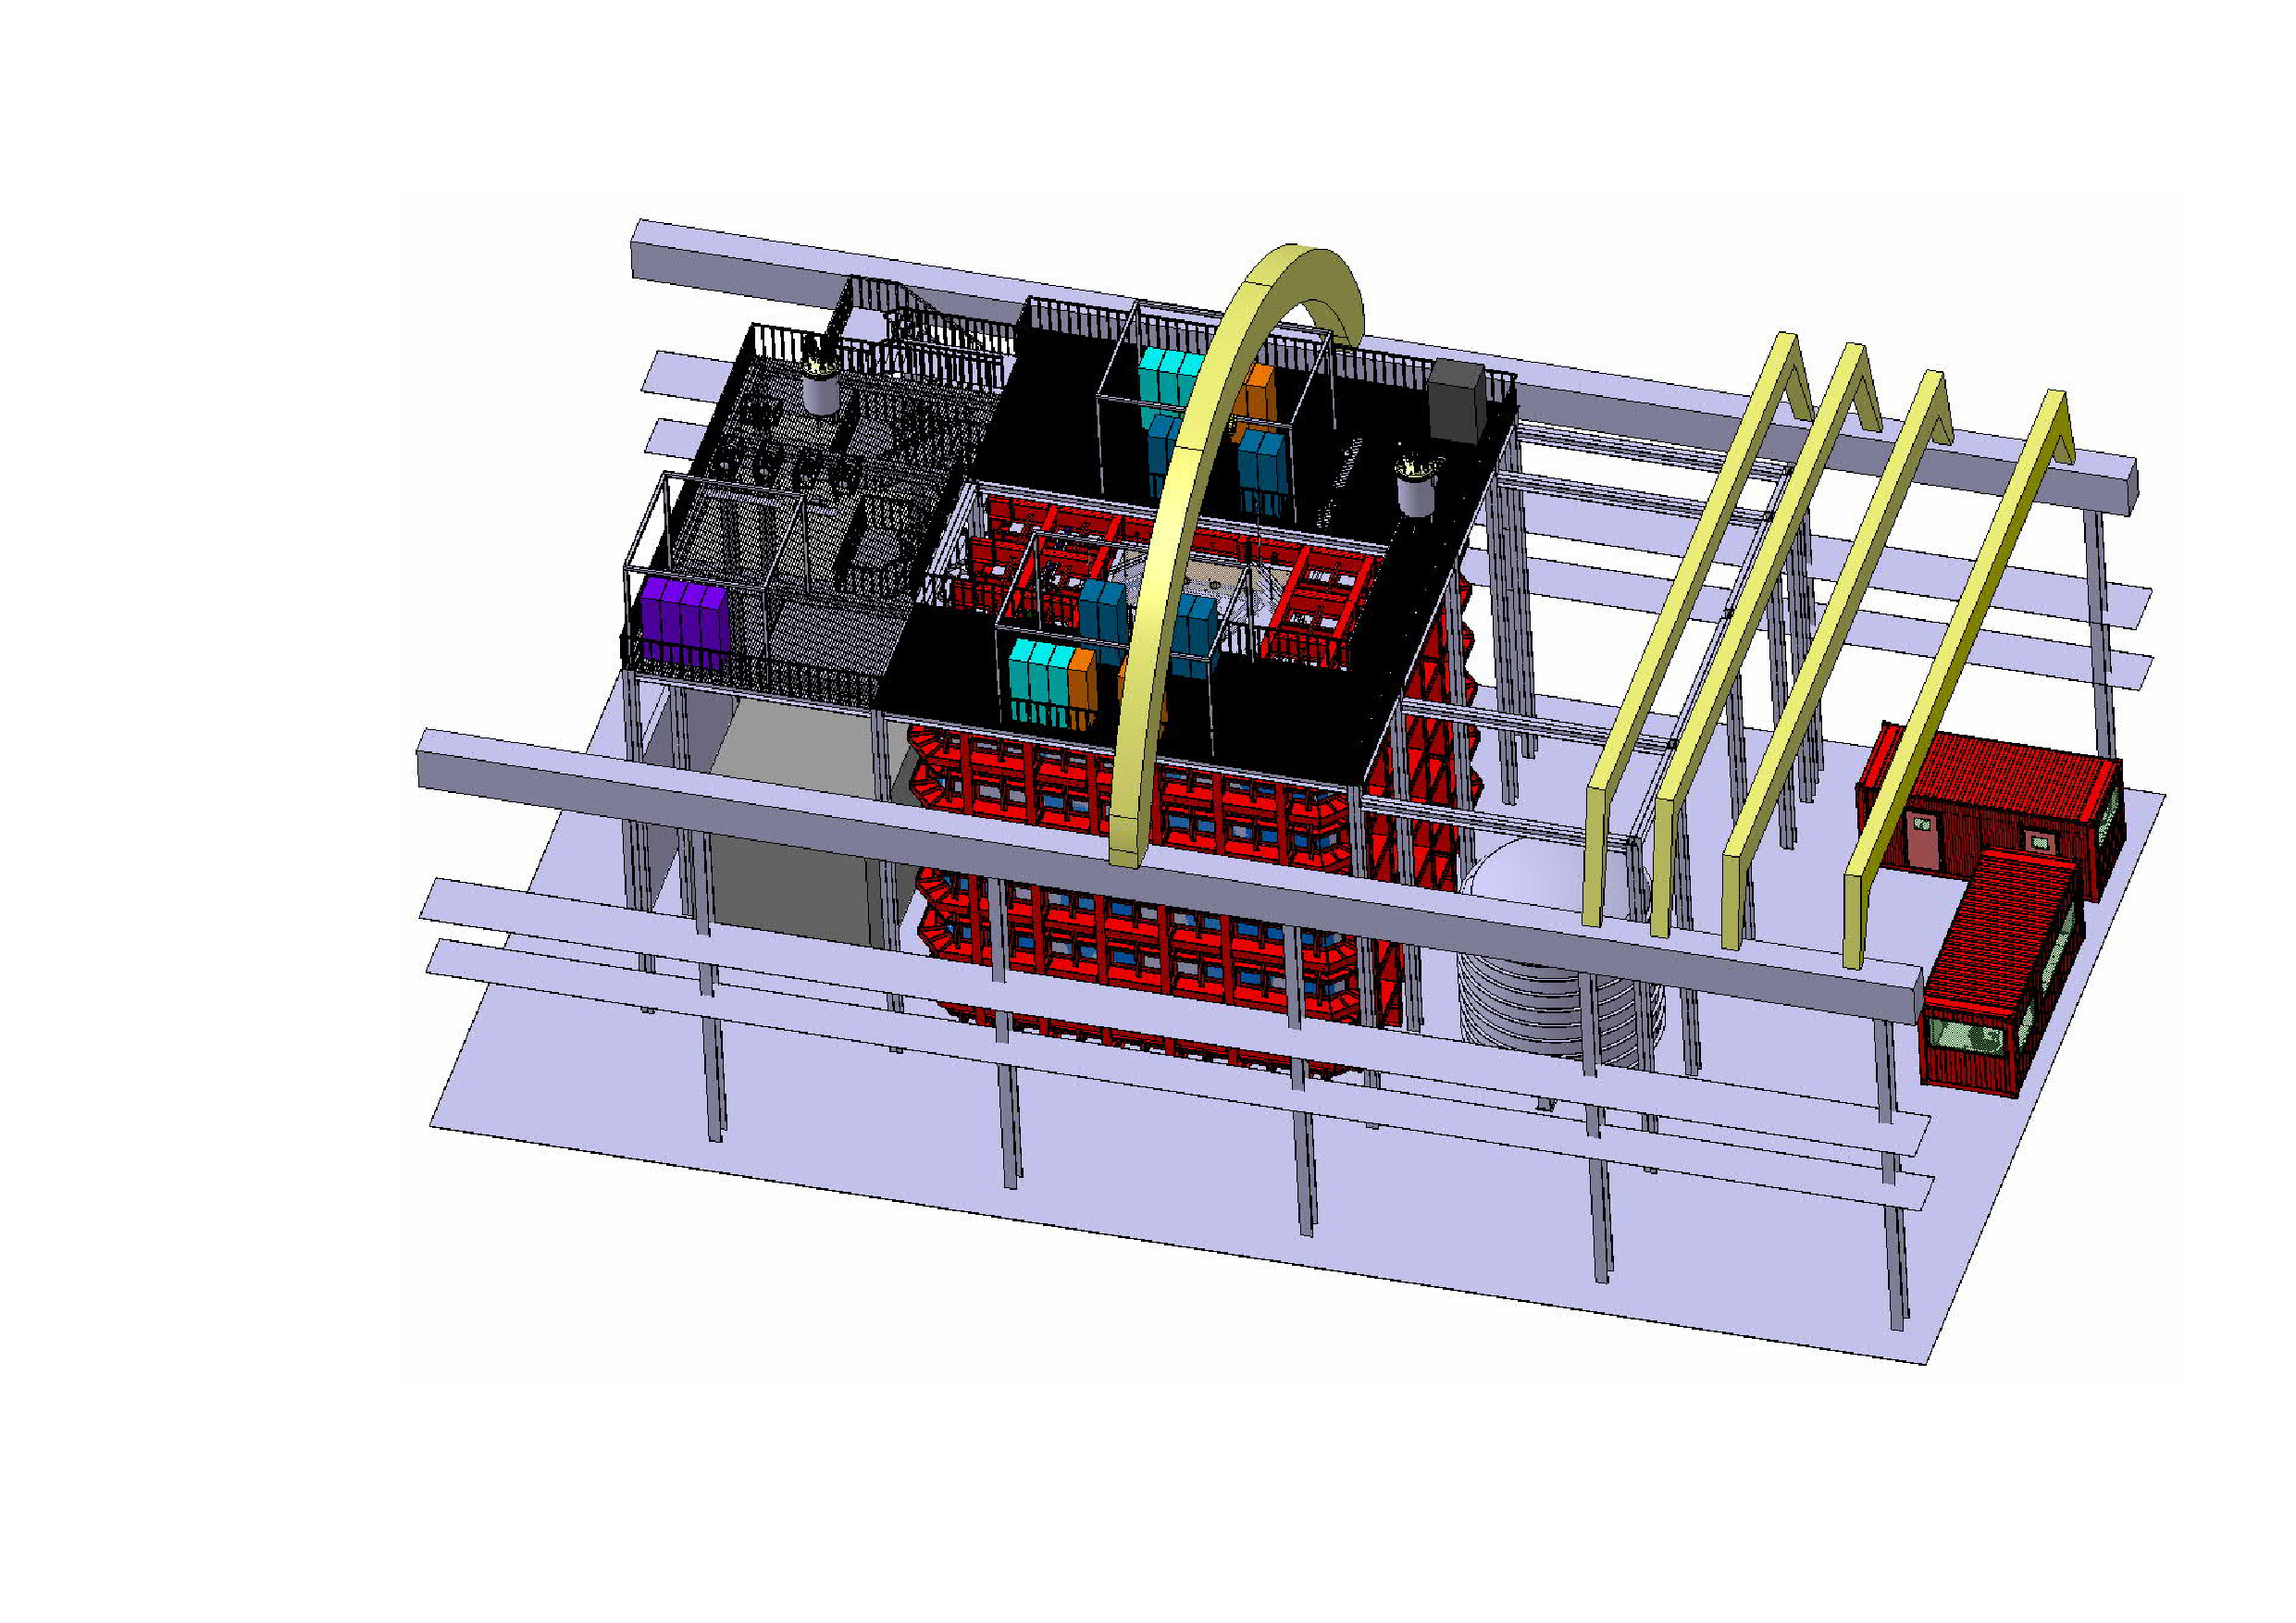
\includegraphics[width=\textwidth]{./Figures/DSk-Overall.pdf}
\caption[Artist rendering of the \DSks\ experiment in Hall C of \LNGS]{Artist rendering of the \DSks\ experiment in Hall C of \LNGS.}
\label{fig:Overall-Design}
\end{figure*}


%---
\subsection{Development Budget and Funding Sources}
The organizations proposing this work, including the sub-award recipients, are all part of two existing collaborative NSF awards that have Princeton as the lead-institution.  The award numbers for the Princeton component are PHY-1812540 and PHY-1622415, but all associated collaborative awards fall within the same scope.  These grants run through 2022 and 2023, respectively, and will cover design and development costs that fall outside of the scope of this Mid-scale RI-1 Program request, but within the same time period.  The first award provides personnel support and operations costs for \DSks\ and the second provides the initial funding for the development and construction of components for \DSks.  Foreign and Domestic partners have received similar grant awards and regional funding to provide the same support for their groups.


%---
\subsection{Development Schedule}
The schedule developed using the Primavera P6 project management system captures activities related to the design and development of the \DSks\ detector components.  It is expected that the first prototype of the \TPC\ will operate in summer of 2019. The \DSp\ (\DSps) 1 tonne-scale prototype will operate in 2020. The Aria facility is currently  in the implementation phase.  The Urania development schedule is set by the ongoing tender process, which will select the contractor to build the plant. A vendor will be selected before the end of 2019: at that point, the final design of the plant will be released by the vendor, and the final schedule for the plant site preparation work will be determined.